% Hasentiles! Hase = zajíc (D)

\section{Wang-tile models}

\subsection{Definition}
	
	% Winfree pg 56
	
	We will rather define Wang tile models less formally because it will be clear what they mean and excessive formality could cause confusions.
	
	Wang tile is a square tile with one color (also index, glue) from a finite nonempty set $I$ on each its edge\footnote{Tiles keep orientation, they are {\em not} allowed to rotate nor reflect.}, let us denote (nonempty) set of all available tiles $T$. Wang tiling is a mapping ${\cal T}: (\Z^2) \rightarrow T$ with restrictions: neighboring tiles must have the same color on the adjacent edge and its domain is required to be (topologically) connected. Wang tiling ${\cal T}_2$ is called {\em reachable} from Wang tiling ${\cal T}_1$ iff ${\cal T}_1 \subseteq {\cal T}_2$. A tiling $\cal T$ is called {\em terminal} iff there does not exist any sharply bigger tiling reachable from $\cal T$. %!% říct jaký to uspořádání je, že má minimální prvek
	
	Winfree extends this definition for DNA tile assembly purposes and introduces Abstract Tile Assembly Model (aTAM). Additionally
	\begin{itemize}
		\item every color $c$ is associated with a nonnegative integer $g(c)$ which will also be referred to as {\em glue strength},
		\item there exists an empty color denoted by $\epsilon$ which can be neighboring with arbitrary color,
		\item tiling is only allowed to grow
		\begin{itemize}
			\item from a special initial tile denoted by $t_0$ from $(0,0)$ ({\em initial configuration}),
			\item one tile per step,
			\item the sum of just connected glues must be greater or equal to given integer treshold\footnote{Interesting to study are small numbers like $1$, $2$; there are different results in Section \ref{sec:wang_power}}, so called {\em temperature}, denoted by $\tau$.
		\end{itemize}
	\end{itemize}
	Reachability relation will be restricted accordingly to these rules, {\em reachable in (tilesystem) $T$} will mean reachable from initial configuration, same for {\em terminal tiling in (tilesystem) $T$}.
	
	Similarly to Turing machines, tilesystem $T$ will be called:
	\begin{description}
		\item[Deterministic] iff there exists unique terminal tiling in $T$. % (in other words, reachability relation has one minimal/maximal member).
		\item[Non-deterministic] iff it has no other restrictions. % no ...
		\item[Probabilistic] iff every possible step in every stage has defined probability. See Note \ref{note:tilesystems} for a proposal how the probability could be defined.
	\end{description}
	
	\begin{note}\label{note:tilesystems}
		If there is a unique place and a unique tile the probability is clearly $1$. If there is a unique place but there are more candidate tiles, the probability $\prob_C(t)$ of connecting tile $t$ should be distributed to these tiles somehow according to their concentration ratio (denoted by $\prob_0(t)$) and their total connectible glue strength (denoted by $G(t)$). Most straightforward is weighted average:
		\begin{equation*}
			\prob_C(t) = \frac{G(t)\cdot\prob_0(t)}{\sum\limits_{u\textnormal{ possible tile}}G(u)\cdot\prob_0(u)}
		\end{equation*}
		In the most general case there are more places, each having several candidates. The probability $\prob_C(t,i)$ of connecting tile $t$ on place $i$ can be defined as weighted average again, now with one more sum over all possible places:
		\begin{equation*}
			\prob_C(t,i) = \frac{G(t,i)\cdot\prob_0(t)}{\sum\limits_{j\textnormal{ possible place}}\quad\sum\limits_{u\textnormal{ possible tile}\atop\textnormal{on place }j}G(u,j)\cdot\prob_0(u)}
		\end{equation*}
	\end{note}

\subsection{Computational power}\label{sec:wang_power}
	
	The most exciting thing about aTAM is that
	\begin{itemize}
		\item it is known to be capable of universal computation at temperature $2$ in 2D,
		\item also at temperature $1$ in 3D,
		\item but it is not known to be universal or not at temperature $1$ in 2D\footnote{Universality has been reached only with modifications to the original model, see \cite{stage_assembly}, \cite{active_tiles}.}.
	\end{itemize}
	Let us show known results in a table.
	
	\begin{center}
	\begin{tabular}{|| c || c | c | c ||}
		\hline\hline
		~ & \multicolumn{2}{c|}{\bf $n\times n$ squares} & {\bf Computational} \\
		~ & \multicolumn{1}{c}{LB} & \multicolumn{1}{c|}{UB} & {\bf Power}\\
		\hline
		$\tau=2$, 2D & \multicolumn{2}{c|}{See \cite{square_lb}, $\Theta(\frac{\log n}{\log\log n})$, see \cite{square_ub}} & Universal, see \cite{winfree_phd} \\
		\hline
		$\tau=1$, 3D & $\Omega(\frac{\log n}{\log\log n})$, see \cite{square_lb} & $O(\log n)$, see \cite{cook_temp1} & Universal, see \cite{cook_temp1} \\
		\hline
		$\tau=1$, 2D & $\Omega(\frac{\log n}{\log\log n})$, see \cite{square_lb} & $2n-1$, see \cite{square_lb} & Unknown \\
		\hline\hline
	\end{tabular}
	\end{center}

\subsection{Turing universality of 2D tiles at $\tau=2$}
	
	Here we propose an alternative and more straightforward 2D tilesystem denoted by ${\cal T}_{TM}$ which directly simulates Turing machine at $\tau=2$ proving Turing universality of this model, see Figures \ref{fig:tileset1} and \ref{fig:tileset2}. All tiles are described within figures.
	\begin{remark}
		This tilesystem can simulate deterministic Turing machine as well as non-deter\-ministic or probabilistic if we consider probabilistic tilesystem, all in $O(1)$ biosteps.
	\end{remark}
	The worst case occurs when the head is changing its step direction because all the rest of the tape must be copied. Following lemma gives upper bound for binding complexity as well as for the other studied complexities.
	\begin{lemma}
	\label{lem:TM_bound}
		Studied complexities in tilesystem ${\cal T}_{TM}$ are bounded:
		\begin{description}
			\item[Biostep] $Bs(n) \in O(1)$.
			\item[Binding] $Bnd(n) \in O(t^2(n))$ where $t(n)$ denotes time of the simulated Turing machine.
			\item[Tile] $Ti(n) \in O(n)$.
			\item[Glue] $Gl(n) \in O(n)$.
		\end{description}
	\end{lemma}
	\begin{proof}
		~
		\begin{description}
			\item[Biostep] all tiles are designed to operate altogether thus only constant number of biosteps is needed.
			\item[Binding] all Turing machine steps are simulated one-to-one or one-to-constant number of bindings with only one exception which is tape-copying as soon as head changes its direction. The length of %!% popsaný
			used tape is $\leq t(n)$. Every copied length is thus bounded by $t(n) + C$ where $C$ is a constant, copying process is thus bounded by $2(t(n)+C)$ bindings. Copying occurs maximally once per simulated step thus number of copying is bounded by $t(n)$. Altogether number of bindings is bounded by $2(t(n)+C)\cdot t(n) \in O(t^2(n))$.
			\item[Tile] number of non-input tiles is constant, it is proportional to Turing machine size which is constant. There must only be prepared $n$ special input tiles thus $Ti(n) \in O(n)$.
			\item[Glue] from Lemma \ref{lem:ti_gl} follows that $Gl(n) \leq 4Ti(n)$ and I really need $n$ glues to connect input tiles uniquely, $Gl(n)\in O(n)$.
		\end{description}
	\end{proof}
	\begin{cor}
	\label{cor:poly_resist}
		All classes resistant to polynomial slowdown ($\P$, $\ZPP$, $\RP$, $\BPP$, $\NP$, \ldots) remain preserved for all studied complexities.
	\end{cor}
	
	\begin{figure}[h]
	\begin{center}
		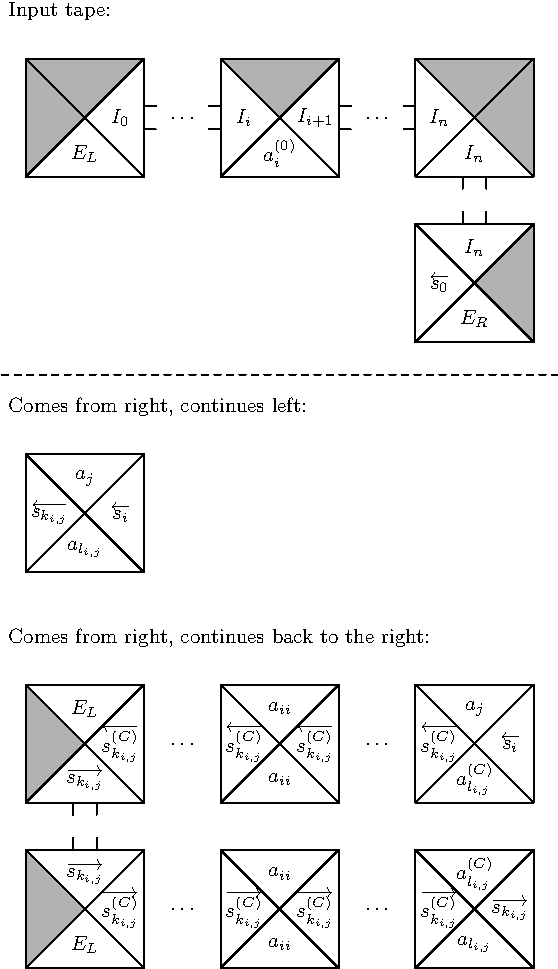
\includegraphics{./figures/tiles1.pdf}
		\caption{Tileset 1/2. Symmetric tiles are considered.}
		\label{fig:tileset1}
	\end{center}
	\end{figure}
	
	\begin{figure}[h]
	\begin{center}
		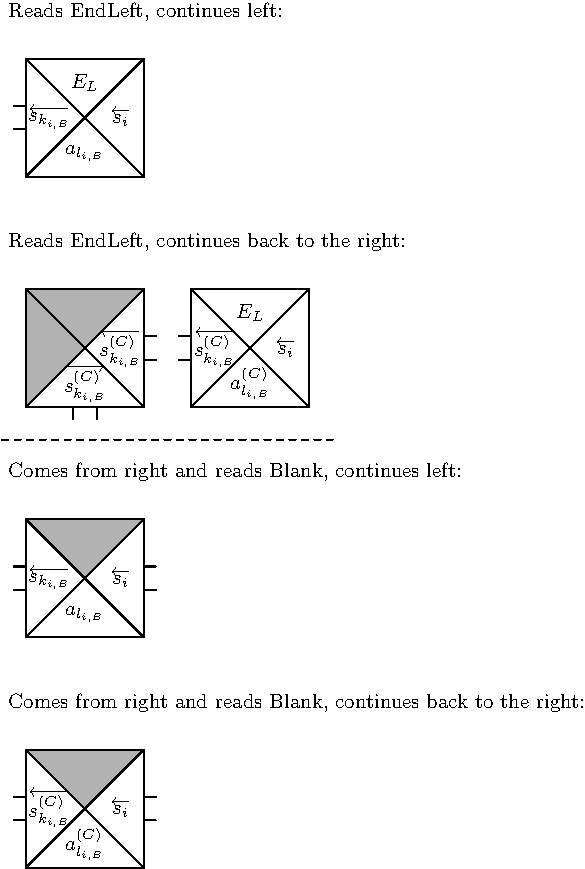
\includegraphics{./figures/tiles2.pdf}
		\caption{Tileset 2/2. Symmetric tiles are considered.}
		\label{fig:tileset2}
	\end{center}
	\end{figure}

\subsection{Feasibility of the class $\BPP$}
	
	Remind that every language from $\BPP$ is dedidable on a PTM in polynomial time which means that probability of correct result is $> \nicefrac{2}{3}$. Note that one can reach probability of correct result higher than arbitrary constant $<1$ by constant number of iterations. Thus it is reasonable to consider $\BPP$ as practically feasible\footnote{Considering even Quantum Turing machine to be practically feasible, $\BQP$ (a superset of $\BPP$) would be practically feasible. Note that due to Shor's algorithm \cite{shor94}, Integer Factorization Problem belongs to $\BQP$ but it is assumed that it does not belong to $\BPP$. Thus $\BPP$ is assumed to be proper subset of $\BQP$.}.
	
	Here we introduce a similar proposal for feasibility of DNA algorithms. In Remark \ref{rem:stud_compl} we proposed that feasible algorithms' biostep complexity must comply $Bs(n)\in O(1)$ which is proved in Lemma \ref{lem:TM_bound} for tilesystem ${\cal T}_{TM}$. There are also practical reasons for limitation of the other complexities, not yet so sharp, so we will require them to be polynomial. Corollary \ref{cor:poly_resist} states preserving of classes $\P$, $\ZPP$, $\RP$, $\BPP$, $\NP$, \ldots in tilesystem ${\cal T}_{TM}$ which justifies Corollary \ref{cor:bpp_feas}.
	
	\begin{thesis}   %!% conjecture nebo lépe?
		Feasible DNA algorithms comply $Bs(n)\in O(1)$; $Bnd(n),\,Ti(n),\,Gl(n)\in \P$.   %!% možná postačí pro poly algoritmus mín jak \P tile a glue !!! ale spíš ne
	\end{thesis}
	
	\begin{cor}
	\label{cor:bpp_feas}
		$\BPP$ is feasible in 2D at temperature $\tau=2$.
	\end{cor}
	
	\begin{note}
		Remind that $\P$, $\ZPP$, $\RP$ and $\coRP \subseteq \BPP$.
	\end{note}
	
	
	
	%~ \begin{thm}   %!% tohle je potřeba někde najít a citovat
		%~ Probabilistic Turing machine can be simulated by probabilistic cellular automaton.
	%~ \end{thm}
	
	%!% popsat co znamená že je něco sestavitelný -- NP, že má něco pst sestavení -- BPP
	
	%!% nák rozumně vysvětlit že \NP se dá na PTM docela dobře spočítat
	% The model can practically handle also $\NP$ languages (not theoretically, of course) because 
	
	%%%%%%%%%%%%%%%%%%%%%%%%%%%%%%%%%%%%%%%%%%%%%%%%%%%%%%%%%%%%%%%%%%%%%%
	
	% error-tolerant rules -- Gacs and Reif, 1988\\
